\section*{1. Uso cotidiano de la PC}
La PC se utiliza principalmente para el desarrollo de software y la ejecución de simulaciones. Los programas y entornos utilizados incluyen:

\begin{itemize}
    \item \textbf{Desarrollo de software:} Visual Studio Code, PyCharm, Eclipse.
    \item \textbf{Simulaciones:} MATLAB, Simulink, ANSYS.
    \item \textbf{Otros:} Navegación web con múltiples pestañas, edición de documentos en \LaTeX.
\end{itemize}

\section*{2. Tareas y benchmarks representativos}

A continuación, se presenta una tabla con algunas tareas frecuentes relacionadas con simulaciones y desarrollo de código, junto con el benchmark que mejor representa cada una.

\begin{center}
\begin{tabular}{|p{7cm}|p{7cm}|}
\hline
\textbf{Tarea} & \textbf{Benchmark representativo} \\
\hline
Compilar proyectos grandes en C/C++ & Geekbench o Cinebench (CPU multi-core) \\
\hline
Ejecución de simulaciones en MATLAB/Simulink & SPEC CPU2017 \\
\hline
Desarrollo de software en entornos pesados (e.g., PyCharm, Eclipse) & PassMark CPU \\
\hline
Análisis de datos y cálculos intensivos en Python & Geekbench (CPU single-core) \\
\hline
\end{tabular}
\end{center}

A continuación se presentan los resultados de la herramienta \textbf{Geekbench}, que permite evaluar el rendimiento general del sistema en distintos escenarios.

\begin{figure}[H]
    \centering
    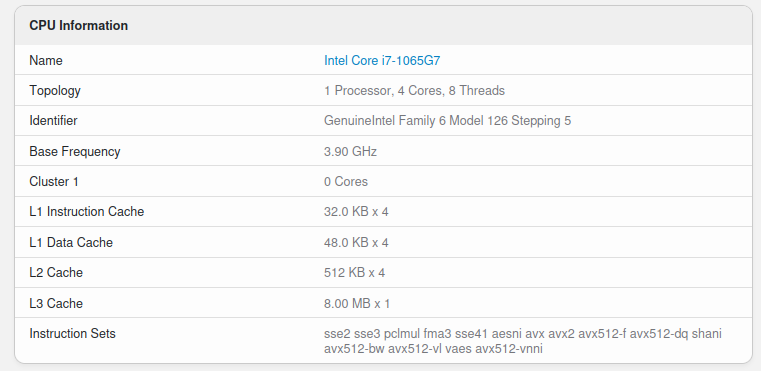
\includegraphics[width=0.7\linewidth]{img/sistema.png}
    \caption{Características del sistema evaluado}
    \label{fig:prestaciones}
\end{figure}

\begin{figure}[H]
    \centering
    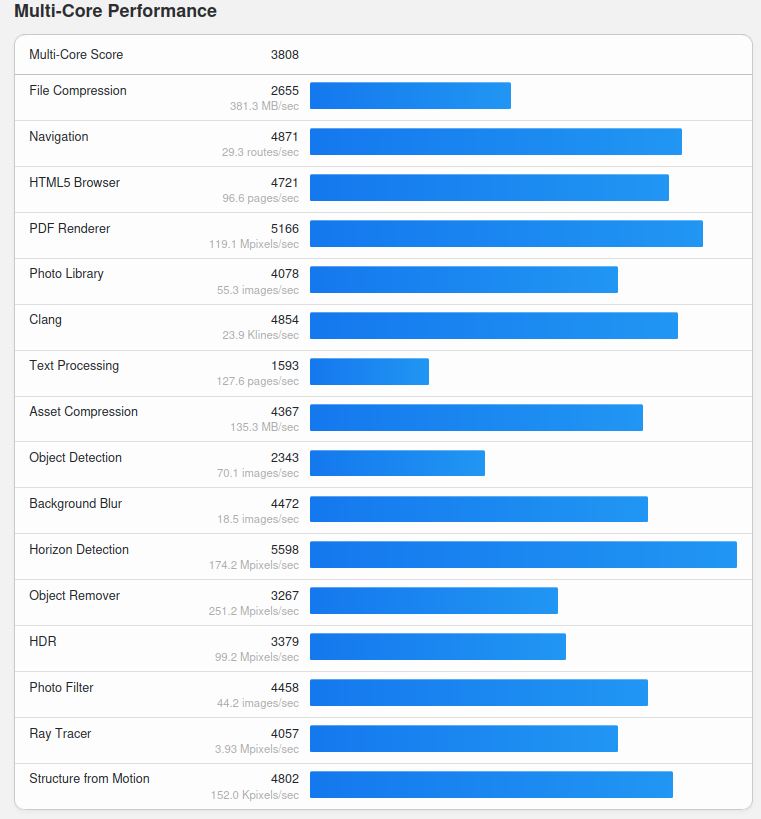
\includegraphics[width=0.7\linewidth]{img/rendimientoGeek.png}
    \caption{Resultados obtenidos con Geekbench}
    \label{fig:resultado-geekbench}
\end{figure}

Como se puede observar, el sistema muestra un buen rendimiento en tareas generales como navegación web, manejo de documentos PDF e imágenes, y edición de texto. Sin embargo, es importante tener en cuenta que los resultados del benchmark podrían haber sido parcialmente afectados, ya que durante su ejecución se estaba instalando software adicional en segundo plano.

Adicionalmente, se intentó ejecutar otros benchmarks como \textbf{SPEC CPU2017} y \textbf{PassMark CPU}, pero no fue posible completar las pruebas debido a que son herramientas de pago o presentan incompatibilidades con la versión actual de Ubuntu utilizada en la máquina evaluada.

\section*{3. Reflexión final}
En términos generales, la PC cumple con los requerimientos diarios para el desarrollo de software y la ejecución de simulaciones. Sin embargo, se ha identificado que el rendimiento de la CPU puede convertirse en un cuello de botella durante la ejecución de simulaciones complejas y la compilación de proyectos grandes.
